\documentclass[tikz,border=10pt]{standalone}
\usepackage{amsmath}
\usepackage{amssymb}
\usepackage{tikz}
\usetikzlibrary{arrows.meta,calc,decorations.pathreplacing,decorations.markings,patterns,shapes.geometric,positioning,shadings,plotmarks}

\begin{document}
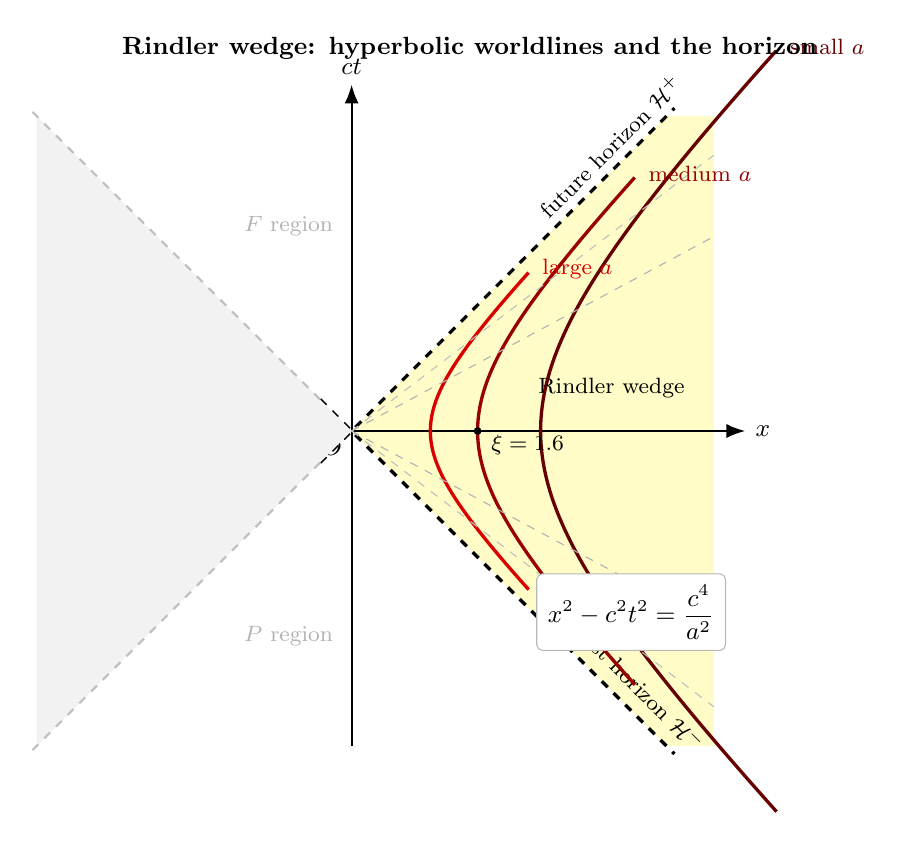
\begin{tikzpicture}[scale=1.0,>={Latex[length=2.4mm]},font=\small]

% =========================================================================
% Rindler diagram in Minkowski (t-x) plane (we use units c=1, so axis is "ct")
% Three uniformly accelerated worldlines (hyperbolae):
%   x^2 - (ct)^2 = a^{-2}    (with c^4/a^2 -> 1/a^2 in units c=1)
% Hyperbola parameter values:  a = 1/r,  with r in {1.0, 1.6, 2.4}
%   ct = r * sinh(eta),  x = r * cosh(eta)   (eta in radians)
% Asymptotes ct = +- x are the Rindler horizons.
% Right wedge (x > |ct|) shaded yellow.
% =========================================================================

\def\xmax{4.6}     % horizontal extent in units of "x" (c=1)
\def\ymax{4.0}     % vertical extent (ct)
\def\etaM{1.45}    % rapidity range so curves stay in box

% -------------------------------------------------------------------------
% (1) Rindler wedge shading (right wedge: x > |ct|, x <= xmax)
% -------------------------------------------------------------------------
\fill[yellow!22]
  (0,0) -- (\ymax, \ymax) -- (\xmax, \ymax) -- (\xmax, -\ymax)
  -- (\ymax, -\ymax) -- cycle;

% -------------------------------------------------------------------------
% (2) Light cone / Rindler horizon (asymptotes ct = +- x), dashed black
% -------------------------------------------------------------------------
\draw[black, dashed, very thick] (-0.4, -0.4) -- ({\ymax+0.1}, {\ymax+0.1});
\draw[black, dashed, very thick] (-0.4,  0.4) -- ({\ymax+0.1}, {-(\ymax+0.1)});

% Horizon labels
\node[font=\footnotesize, rotate=45, anchor=south]
  at ({\ymax-0.55}, {\ymax-0.55}) {future horizon $\mathcal{H}^{+}$};
\node[font=\footnotesize, rotate=-45, anchor=south]
  at ({\ymax-0.55}, {-(\ymax-0.55)}) {past horizon $\mathcal{H}^{-}$};

% -------------------------------------------------------------------------
% (3) Coordinate axes (drawn over the wedge fill)
% -------------------------------------------------------------------------
\draw[->, thick] (-0.4, 0) -- ({\xmax+0.4}, 0) node[right] {$x$};
\draw[->, thick] (0, -\ymax) -- (0, {\ymax+0.4}) node[above] {$ct$};
\node[below left, font=\footnotesize] at (0,0) {$O$};

% -------------------------------------------------------------------------
% (4) Three hyperbolic worldlines (different proper acceleration a)
%     parameterized as  x = r cosh(eta),  ct = r sinh(eta),  r = 1/a
% -------------------------------------------------------------------------

% Hyperbola 1: r = 1.0 (large a)
\draw[red!85!black, very thick, smooth, samples=80, domain=-\etaM:\etaM]
  plot ({1.0*cosh(\x)}, {1.0*sinh(\x)});

% Hyperbola 2: r = 1.6 (medium a)
\draw[red!60!black, very thick, smooth, samples=80, domain=-\etaM:\etaM]
  plot ({1.6*cosh(\x)}, {1.6*sinh(\x)});

% Hyperbola 3: r = 2.4 (small a)
\draw[red!40!black, very thick, smooth, samples=80, domain=-\etaM:\etaM]
  plot ({2.4*cosh(\x)}, {2.4*sinh(\x)});

% -------------------------------------------------------------------------
% (5) Constant-eta lines (Rindler "time slices" through O)
%     ct = x tanh(eta_0), restricted to right wedge
% -------------------------------------------------------------------------
\foreach \eta/\sty in {0.6/{gray!60}, -0.6/{gray!60}, 1.0/{gray!50}, -1.0/{gray!50}}{
  \draw[\sty, thin, dashed]
    (0,0) -- ({\xmax}, {\xmax*tanh(\eta)});
}

% -------------------------------------------------------------------------
% (6) Mark a typical event on the middle hyperbola at eta = 0
% -------------------------------------------------------------------------
\fill[black] (1.6, 0) circle (1.4pt);
\node[font=\footnotesize, anchor=west] at (1.65, -0.18) {$\xi = 1.6$};

% -------------------------------------------------------------------------
% (7) Labels for the hyperbolae (right edge)
% -------------------------------------------------------------------------
\node[red!85!black, font=\footnotesize, anchor=west]
  at ({1.0*cosh(\etaM)+0.05}, {1.0*sinh(\etaM)+0.05}) {large $a$};
\node[red!60!black, font=\footnotesize, anchor=west]
  at ({1.6*cosh(\etaM)+0.05}, {1.6*sinh(\etaM)+0.05}) {medium $a$};
\node[red!40!black, font=\footnotesize, anchor=west]
  at ({2.4*cosh(\etaM)+0.05}, {2.4*sinh(\etaM)+0.05}) {small $a$};

% -------------------------------------------------------------------------
% (8) Wedge label and equation box
% -------------------------------------------------------------------------
\node[font=\footnotesize, anchor=center]
  at (3.3, 0.55) {Rindler wedge};

\node[draw=gray!55, fill=white, rounded corners=2pt, inner sep=4pt, font=\small]
  at (3.55, -2.3)
  {$x^{2}-c^{2}t^{2}=\dfrac{c^{4}}{a^{2}}$};

% -------------------------------------------------------------------------
% (9) Forbidden / inaccessible regions outside right wedge - light gray
% -------------------------------------------------------------------------
\node[font=\footnotesize, gray!60, rotate=0]
  at (-0.8, 2.6) {$F$ region};
\node[font=\footnotesize, gray!60, rotate=0]
  at (-0.8, -2.6) {$P$ region};
\node[font=\footnotesize, gray!60, rotate=0]
  at (-2.2, 0) {$L$ wedge};

% Mark "L" wedge on the left (mirror Rindler wedge), with hatched fill
\fill[gray!10]
  (0,0) -- (-\ymax, \ymax) -- (-\xmax+0.6, \ymax) -- (-\xmax+0.6, -\ymax)
  -- (-\ymax, -\ymax) -- cycle;
\draw[gray!50, dashed, thick] (-0.4, 0.4) -- ({-(\ymax+0.1)}, {\ymax+0.1});
\draw[gray!50, dashed, thick] (-0.4, -0.4) -- ({-(\ymax+0.1)}, {-(\ymax+0.1)});

% -------------------------------------------------------------------------
% (10) Caption-like header above figure
% -------------------------------------------------------------------------
\node[font=\bfseries\small, anchor=south]
  at (1.5, {\ymax+0.6}) {Rindler wedge: hyperbolic worldlines and the horizon};

\end{tikzpicture}
\end{document}
